%%%%%%%%%%%%%%%%%%%%%%%%%%%%%%%%%%%%%%%%%
% University/School Laboratory Report
% LaTeX Template
% Version 3.1 (25/3/14)
%
% This template has been downloaded from:
% http://www.LaTeXTemplates.com
%
% Original author:
% Linux and Unix Users Group at Virginia Tech Wiki 
% (https://vtluug.org/wiki/Example_LaTeX_chem_lab_report)
%
% License:
% CC BY-NC-SA 3.0 (http://creativecommons.org/licenses/by-nc-sa/3.0/)
%
%%%%%%%%%%%%%%%%%%%%%%%%%%%%%%%%%%%%%%%%%

%----------------------------------------------------------------------------------------
%	PACKAGES AND DOCUMENT CONFIGURATIONS
%----------------------------------------------------------------------------------------

\documentclass{article}

\usepackage[version=3]{mhchem} % Package for chemical equation typesetting
\usepackage{siunitx} % Provides the \SI{}{} and \si{} command for typesetting SI units
\usepackage{graphicx} % Required for the inclusion of images
\usepackage{natbib} % Required to change bibliography style to APA
\usepackage{amsmath} % Required for some math elements 

\setlength\parindent{0pt} % Removes all indentation from paragraphs

\renewcommand{\labelenumi}{\alph{enumi}.} % Make numbering in the enumerate environment by letter rather than number (e.g. section 6)

%\usepackage{times} % Uncomment to use the Times New Roman font

%----------------------------------------------------------------------------------------
%	DOCUMENT INFORMATION
%----------------------------------------------------------------------------------------

\title{High Performance Programming with Multicore \& GPU \\ Final Project \\ Professor Herbordt} % Title

%\author{Ryan \textsc{Lader}} % Author name
\author{Luke Sorenson\and Ryan Lader \and Katie Lewis}

\date{\today} % Date for the report

\begin{document}

\maketitle % Insert the title, author and date

% If you wish to include an abstract, uncomment the lines below
% \begin{abstract}
% Abstract text
% \end{abstract}

%----------------------------------------------------------------------------------------
%	SECTION 1
%----------------------------------------------------------------------------------------
\section{Introduction}
Throughout this course, we have studied several algorithms and methods of obtaining optimal performance by using optimization techniques - serial optimizations, multithreading, and GPU. For this project we optimized two learning algorithms: Perceptron, and K-Nearest Neighbors. Perceptron works as a supervised machine learning algorithm for binary classifiers. The algorithm determines whether an input belongs to a distinct class A or B. Perceptron works to perfectly separate data or until convergence occurs. KNN, on the other hand, is an instance-based or ``lazy learning'' algorithm that compares every new piece of data to all of the labeled data, computing some distance between the points, and determining its class based on the nearest labeled data. For Perceptron, we were wrote a serial implementation in C based off MATLAB code, multithread it using PThreads, and transfered the code onto the GPU using both CUDA and OpenCL. K-Nearest Neighbors was written serially in C++ and multithreaded using PThreads as well. These algorithms lend themselves to parallelization because they are highly iterative and perform independent operations on the training data. \\
\\
For all serial and multithreaded tests performed for this report, we used the following machine specifications: \\
\begin{verbatim}
Architecture:          x86_64
CPU op-mode(s):        32-bit, 64-bit
Byte Order:            Little Endian
CPU(s):                12
On-line CPU(s) list:   0-11
Thread(s) per core:    1
Core(s) per socket:    6
Socket(s):             2
NUMA node(s):          2
Vendor ID:             GenuineIntel
CPU family:            6
Model:                 45
Stepping:              7
CPU MHz:               1200.000
BogoMIPS:              4999.29
Virtualization:        VT-x
L1d cache:             32K
L1i cache:             32K
L2 cache:              256K
L3 cache:              15360K
NUMA node0 CPU(s):     0-5
NUMA node1 CPU(s):     6-11
\end{verbatim}

 
%----------------------------------------------------------------------------------------
%	SECTION 2
%----------------------------------------------------------------------------------------
\clearpage
\section{Perceptron - An Overview}
The Perceptron algorithm was first implemented in the 1950s in custom hardware as one of the first artificial neural networks. Put simply, the algorithm visualized best resembles the ``atom'' of the neural network: a single, simple neuron that can answer decision problems (yes or no, black or white, etc). Perceptron maps a real-valued vector, x, to a binary output f(x) such that the dot product x dot w maps to either 1 or -1 (in the context of our data, class A or B). We iteratively update the weight vector based on if the output of the training set is correctly classified or misclassified. The parameter ``eta'' acts as a learning rate, controlling how much the weight vector changes with each misclassified data point.

\begin{figure}[!htbp]
\begin{center}
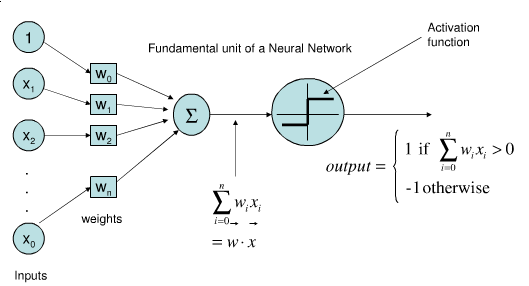
\includegraphics[width=1.0\textwidth]{PerceptronAnimation} % Include the image placeholder.png
\caption{Perceptron Animation}
\end{center}
\end{figure}

Our first step was to migrate a MATLAB implementation over to C to begin optimizing. \\ \\
Serial code:
This portion of the code initializes the array of weights and the array of misclassified flags. We set a flag not\_classified so we know when to exit the main while loop.
\begin{verbatim}
int train_perceptron(data_t* x, char* y, double eta, int x_length, int x_dim) {
    double w[x_dim];
    double score[x_length];
    char misclassified[x_length];
    char not_classified = 1;
    int i, j, sum_missed, iters = 0;
    //set w to 0's, misclassified to 1's
    memset(w, 0, x_dim*sizeof(double));
    memset(misclassified, 1, x_length*sizeof(char));
}
\end{verbatim}
Moving forward to the updating of weights within the while loop:
\begin{verbatim}
while(not_classified && iters <= MAX_ITERS){
        iters++;
        not_classified = 0;
        for(i=0; i < x_length; ++i){
            if(misclassified[i] == 1){
                for(j=0; j< x_dim; ++j){
                    w[j] = w[j] + eta*x[i*x_dim + j]*y[i];
                }
            }
        }
\end{verbatim}
This step simply performs a check and update; if a data point is misclassified, we loop through the weight vector and error-correct it based on the above formula. In the serial implementation, this one double for loop updates all indices of the weight vector using all of the data.
\\ \\
Lastly, the classification step in the main loop:
\begin{verbatim}
 sum_missed = 0;
        for (i=0; i<x_length; ++i) {
            score[i] = 0;
            for (j = 0; j < x_dim; j++) {
                score[i] += x[i*x_dim + j]*w[j];
            }
            misclassified[i] = score[i]*y[i] <= 0.0 ? 1 : 0;
            // Set not_classified to 1 if any data point is misclassfied
            // and count number of missed.
            if (misclassified[i] == 1) {
                sum_missed++;
                not_classified = 1;
            }
        }
\end{verbatim}
In this section of code, we take the dot product of x and w to determine what class our data point belongs to. If we are still misclassified, we increment sum\_missed and set the flag not\_classified to know that we need to continue on to another iteration.
\\ \\
We at first visualized Perceptron using a smaller data set which classifies data based on three different test cases. 
\\ \\ \\ \\
\textbf{Test Case 1 (Separated by a Line) - Code} 
\begin{verbatim}
case 1:
                y[i] = (0.2*(x[i*x_dim + 1] - 0.5)) +
                    (.6-x[i*x_dim + 2]) > 0 ? 1 : -1;
                break;
\end{verbatim}
\textbf{Test Case 2 (Separated by an Oval) - Code} 
\begin{verbatim}
 case 2:
                y[i] = (x[i*x_dim + 1]-.5)*(x[i*x_dim + 1]-.5) +
                    (x[i*x_dim + 2]-.5)*(x[i*x_dim + 2]-.5)
                    > 0.09 ? 1 : -1;
                break;
\end{verbatim}
\textbf{Test Case 3 (Separated by an Parabola) - Code}
\begin{verbatim}
case 3:
                y[i] = 4*(x[i*x_dim + 1]-.5)*(x[i*x_dim + 1]-.5) +
                    (.2-x[i*x_dim + 2]) > 0 ? 1 : -1;
                break;
\end{verbatim}

\begin{figure}[!htbp]
\begin{center}
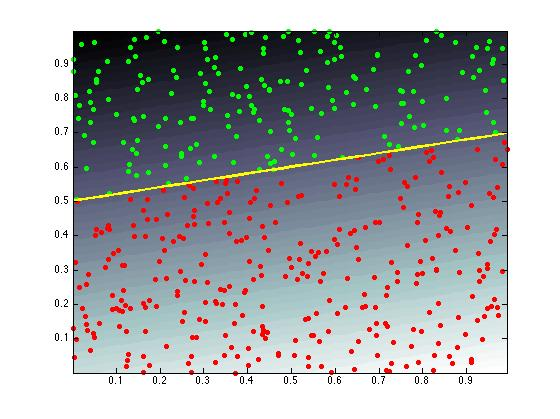
\includegraphics[width=1.0\textwidth]{testcase1.jpg} % Include the image placeholder.png
\caption{Test Case 1 Visualized}
\end{center}
\end{figure}

\begin{figure}[!htbp]
\begin{center}
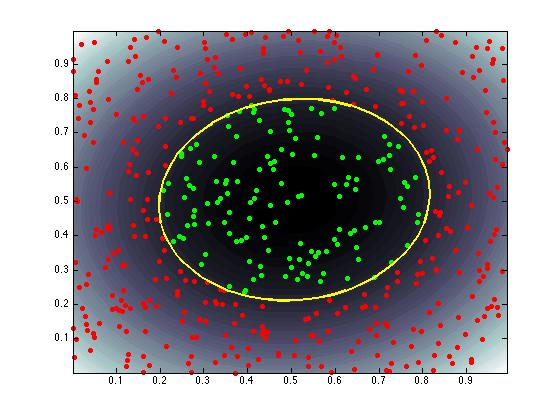
\includegraphics[width=1.0\textwidth]{testcase2.jpg} % Include the image placeholder.png
\caption{Test Case 2 Visualized}
\end{center}
\end{figure}

\begin{figure}[!htbp]
\begin{center}
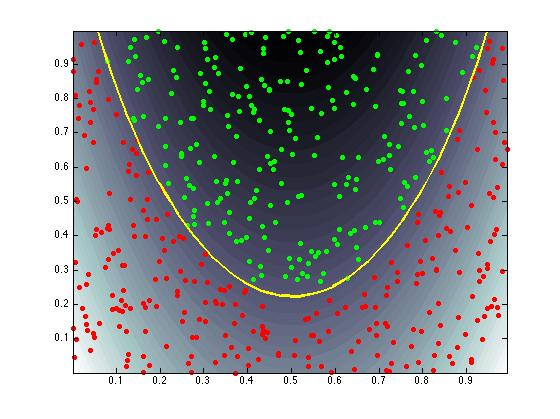
\includegraphics[width=1.0\textwidth]{testcase3.jpg} % Include the image placeholder.png
\caption{Test Case 3 Visualized}
\end{center}
\end{figure}

We performed several operations to preprocess our data before running the algorithm in order to achieve better separation results. Computing $xy$, $x*x$, and $y*y$ allows us to not only separate the 2 dimension data by line but also a parabola or ellipse. 

\begin{figure}[!htbp]
\begin{center}
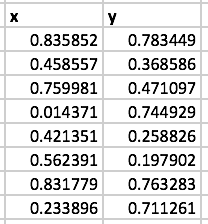
\includegraphics[width=.3\textwidth]{XY.png} % Include the image placeholder.png
\caption{X, Y data generated randomly as values between 0 and 1.}
\end{center}
\end{figure}

\begin{figure}[!htbp]
\begin{center}
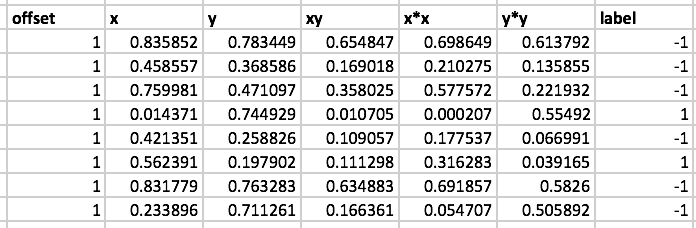
\includegraphics[width=1.0\textwidth]{XYProcessed.png} % Include the image placeholder.png
\caption{Data after processing it to increase the dimensionailty and allow the perceptron algorithm to separate not just along a line.}
\end{center}
\end{figure}


%PREPROCESSED DATA GOES HERE

%----------------------------------------------------------------------------------------
%	SECTION 3
%----------------------------------------------------------------------------------------
\clearpage
\section{Perceptron - Parallelization at a Glance}
To parallelize the Perceptron, we could utilize either task or data parallelism. To elaborate, using task parallelism would involve having each thread operate on the data using a different ``eta'' value to better explore the space. In order to achieve a significant performance improvement for our test case, we needed to use data parallelism by having each thread operate and error correct on a portion of the weight vector in global memory. For this learning algorithm, we expect the accuracy of the results to decrease with datasets that are not completely separable within the provided dimensions and would require some transformation of the data to be able to separate the two classes with a single weight vector.

\section{Perceptron - Multithreading with PThreads}
The goal of this section of optimizing Perceptron was to utilize multi-core architecture in order to improve performance of the training phase of the perceptron algorithm. Each thread will operate on some number of indices of the global weight vector, and hence will require synchronization between threads. The question is whether or not the synchronization implementation is worth the overhead to parallelize the code. Multithreading the code requires the use of several global variables, mutexes, and barriers. Global variables include:
\\ \\
global\_w - Global weight vector that will be updated at each iteration in the master loop. Each thread operates on some number of indices. For example, if we have eight threads and a dimensionality of 24, each thread will update three indices of the global weight vector. \\ \\
global\_not\_classified - A flag that is shared between threads and checked each iteration by every thread order to ensure no threads escape the master loop before we finish classification. \\ \\ 
global\_sum\_missed and global\_countCheck - Counters used to assert that all threads finish classifying the data with no missed classifications. \\ \\
We must set barriers when reading or writing to global\_not\_classified and global\_sum\_missed to ensure no stray threads get stuck in the main loop of the helper function. \\ \\
Perceptron, much like SOR, requires synchronization between threads at every iteration of the main while loop. We must immediately wait for all threads to start the loop together, wait for all threads to finish updating the weight vector before we can begin re-classifying the data, and wait for all threads to finish changing the global variables (which represent critical sections of code). Hence, the multithreaded version of Perceptron requires a considerable amount of overhead and we expect that it may not reach a breakeven point with the serial implementation until the data set becomes quite large.

\begin{verbatim}
 95         // each thread updates one index of the weight vector.
 96         for(i = 0; i < X_length; ++i){
 97             if(misclassified[i] == 1){
 98                 w += eta*X[i*(X_dim) + taskid]*y[i];
 99             }
100         }
101         // each thread updates global weight vector.
102         global_w[taskid] += w;
\end{verbatim}
The code above shows the update step from the multithreaded perceptron implementation. We can see that each index of the weight vector is handled by a separate thread in parallel. For cases where the dimensionality exceeds the available number of CPU cores in the architecture, each thread may handle more than one index of the global weight vector. Here, when the number of misclassified items is small, the amount of work done by each thread will be very small also. At this point in the training, the overhead of synchronizing the threads makes the serial implementation perform better.

\begin{verbatim}
107         // each thread classifies 1/NUM_THREADS of the data.
108         sum_missed = 0;
109         not_classified = 0;
110         local_idx = 0;
111         for (i = X_length_low; i<X_length_high; ++i){
112             score[local_idx] = 0;
113             for(j = 0; j < X_dim; ++j){
114                 score[local_idx] += X[i*(X_dim) + j]*global_w[j];
115             }
116 
117             misclassified[i] = score[local_idx]*y[i] <= 0.0 ? 1 : 0;
118             // Set not_classified to 1 if any data point is misclassfied
119             // and count number of missed.
120             if (misclassified[i] == 1) {
121                 sum_missed++;
122                 not_classified = 1;
123             }
124             local_idx++;
125         }
\end{verbatim}
In the classfication step, the training data is split between threads instead of splitting up the weight vector. This allows each thread to compute the new classifications of a 1/NUM\_THREADS portion of the data, each doing so in parallel. Just as with the update step, when this thread finishes it must wait for all of the other threads to finish as well.

\clearpage
\section{Perceptron - OpenCL and CUDA }
In addition to the serial and pthread code, we also implemented Perceptron on the GPU for optimal speedup and parallelization. We implemented CUDA and OpenCL code to utilize the NVIDIA Tesla M2070 GPU device on scc1. While CUDA was developed by NVIDIA for parallel programming on GPUs, OpenCL is a framework that allows programs to run on heterogeneous devices. Because OpenCL is less specific to the GPU architecture, we expect the OpenCL execution time to be slower than the CUDA execution times, but faster than the CPU versions.
\\ \\
The CUDA and OpenCL implementations of Perceptron use two kernels: calculate\_weights and classify. In both cases, the data is split amongst threads (CUDA) or work-items (OpenCL). For all data sizes, we used a set dimension of 300 threads/work-items per block/work-group. In the first kernel, each thread or work-item computes the weight vector for its assigned row of data if the data is misclassified. The weights are stored in a shared (CUDA) or local (OpenCL) vector, which is accumulated and copied into a weight matrix in the host. Within the host, the weight vectors from each block (CUDA) or work-group (OpenCL) are combined into an overall weight vector. The second kernel, classify, uses the overall weight vector to generate a score and determine whether each data point was correctly classified. Within the classify kernel, each thread or work-item calculates a score and updates the global misclassified and not\_classified arrays. 
\\ \\
To ensure synchronization and concurrency, we used several functions in both the kernel and host code. For CUDA, we used \_\_syncthreads() to synchronize threads within a block, and cudaDeviceSynchronize() to synchronize the blocks in between kernel calls. In OpenCL, we used barrier(CLK\_LOCAL\_MEM\_FENCE) to ensure all work-items ``see'' the same local data (i.e. to maintain concurrency). Within the host code, the clFinish() command prevents host code from executing until all work-groups have finished running the kernel. 
\\ \\
To verify our all of our implementations for training the perceptron, we computed the dot product of the resulting weight matrix with the x vector and checked if the data was correctly classified or not. In all cases, the classifications matched and we were able to completely separate the data into the two fabricated classes (from the assigning labels manually).

\clearpage
\section{Perceptron - Experiments and Results}
We first tested the Perceptron on a small data set of 500 points and 6 dimensions (according to our preprocessing shown above) in order to verify that our code was working, and to graphically visualize our results. Moving on, we began testing our serial algorithm with -O3 optimization against three different implementations of Perceptron: multithreading with PThreads, and GPU implementations using CUDA and OpenCL. Our training set size ranged from 600 to 8000 data points. We modeled the execution time(s) as a function of the number of data points tested. As shown in Figure XXX, the serial version grows faster than the three parallel implementations, and appears to diverge from the bottom three curves. This is expected, as the classifications are very easily separable and require fewer iterations to converge to a solution. The speedups achieved for variable number of data points are as follows:

\begin{figure}[!htbp]
\begin{center}
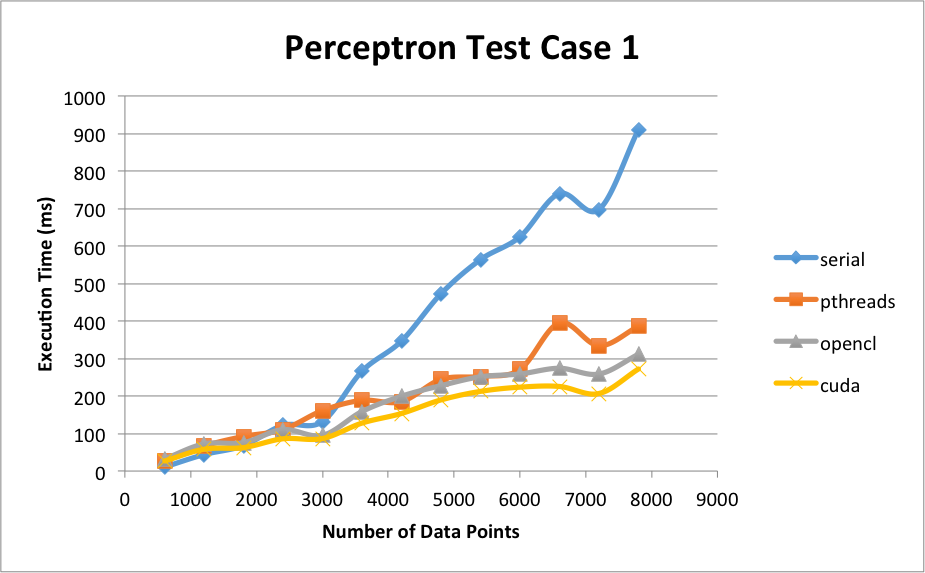
\includegraphics[width=1.0\textwidth]{PerceptronTestCase1} % Include the image placeholder.png
\caption{Perceptron Test Case 1}
\end{center}
\end{figure}
\clearpage
\begin{figure}[!htbp]
\begin{center}
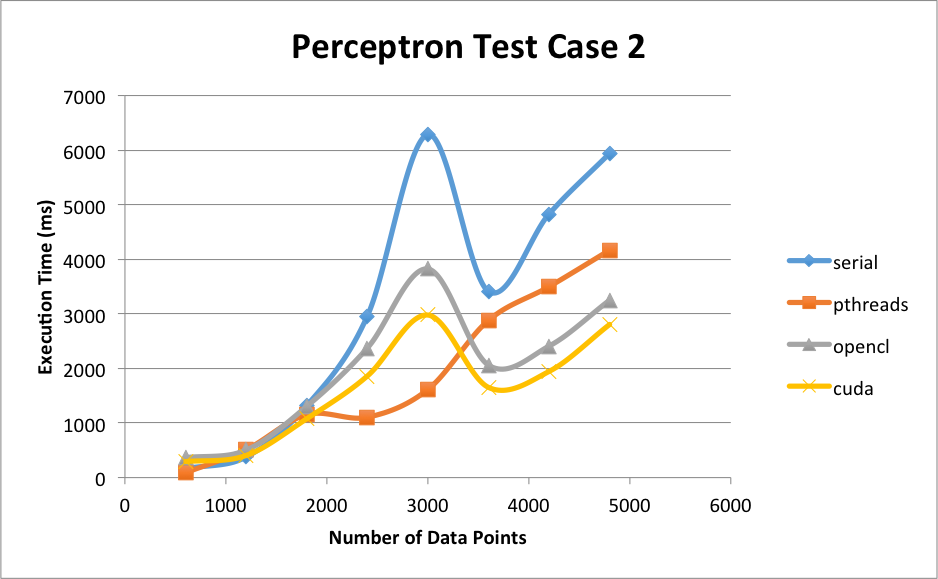
\includegraphics[width=1.0\textwidth]{PerceptronTestCase2} % Include the image placeholder.png
\caption{Perceptron Test Case 2}
\end{center}
\end{figure}

In this this test case (2), we separate the data by an oval. The number of iterations required to perfectly separate the data was on average significantly more than for the first test case. At data size 3000, the spike in the chart is due to an increased number of iterations required to perfectly separate the data (for these tests we did not look at convergence of the number of misclassified data points). The performance improvement for pthreads, OpenCL, and CUDA is not nearly as significant for this test case, because of the larger number of iterations. As the number of iterations grows, so does, generally speaking, the number of classified items. The overhead of synchronization between the parallel implementations then outweighs the benefits of separating the update and classification steps of the global weight vector. The alleviate this problem, we could simply end a pthread or GPU block?s existence when the number of misclassified elements it?s responsible for is small. However, making this modification occur at the right point in time for each thread would require quite a few tests to determine the overhead of running on N threads versus N/2 threads, for example. Furthermore, this would significantly increase the complexity of synchronization between threads and harder to achieve a verifiably correct result.
\clearpage
\begin{figure}[!htbp]
\begin{center}
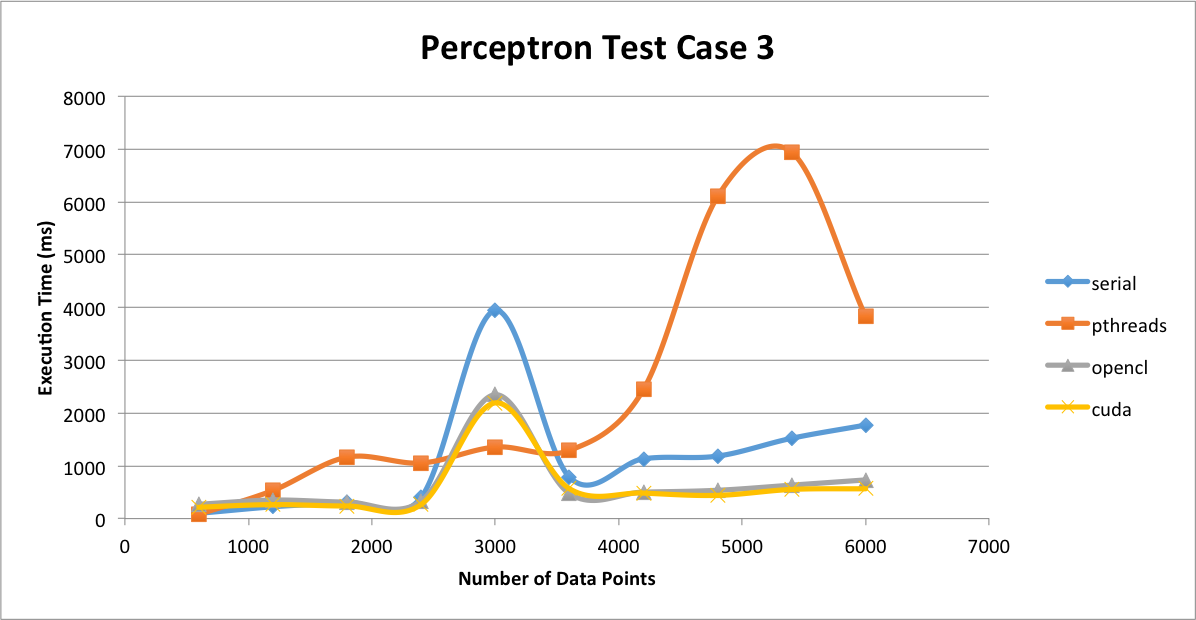
\includegraphics[width=1.0\textwidth]{PerceptronTestCase3} % Include the image placeholder.png
\caption{Perceptron Test Case 3}
\end{center}
\end{figure}

In this last test case (separated by a parabola), we see that for large data sizes the pthreads implementation takes longer than the serial version. The number of iterations required to get to perfect separation increases significantly for the pthreads implementation, but not at a data size of 3000, as it does with the serial and GPU implementations.
\\ \\
\begin{tabular}{ |p{3cm}||p{3cm}|p{3cm}|p{3cm}|  }
 \hline
 \multicolumn{4}{|c|}{Perceptron: Average Speedup Over Serial Version} \\
 \hline
 & Test Case 1 & Test Case 2 & Test Case 3\\
 \hline
 PThreads & 2.148 & 1.572 & 1.750\\
 CUDA & 2.587 & 1.943 & 1.961\\
 OpenCL & 1.841 & 1.683 & 0.459\\
 \hline
\end{tabular}
\clearpage
\section{K-Nearest Neighbors - An Overview}
K-Nearest Neighbors is a lazy algorithm that classifies any new data point based on existing labeled data. A new point is compared to every labeled data point with some distance metric, for example euclidean or hamming distance. The K-nearest neighbors vote on the classification of the new data point by performing a mode operation. K-nearest neighbors, while unlike other machine learning algorithms in that the time it takes to classify a single data point grows with the number of training items, is still widely used to solve problems that are not well-understood or patterns are not intuitive. For example, K-nearest neighbors has been used to diagnose breast cancer from mammograms by comparing a new screening with a set of labeled mammograms. For KNN, we implemented a serial version of the code based on a MATLAB implementation and also a pthread implementation. We wanted to apply both KNN and perceptron to a real world dataset to compare running times and also accuracy for these two simple algorithms. 
% why is this here, (http://citeseerx.ist.psu.edu/viewdoc/download?doi=10.1.1.303.6019&rep=rep1&type=pdf)
\\ \\
For KNN we used a dataset found on the UCI Machine Learning Repository, 
%http://archive.ics.uci.edu/ml/datasets/default+of+credit+card+clients 
which has 23 attributes about each credit card holder and whether or not they defaulted on their next payment. It is an interesting application of machine learning, which may have practical relevance to a credit card issuer, that without spending a considerable amount of time understanding the various dimensions of the data is not immediately obvious that we would be able to achieve any accuracy at all. Still, we were able to apply KNN on the raw data from the dataset and achieve a classification rate of up to 78.5\%. With Perceptron, we could not perfectly separate the raw data with a linear weight vector (this is where neural nets would come in), but we were able to converge to a correct classification rate of 78.8\%. It is somewhat surprising that either algorithm would have any success at all on this data.
\begin{verbatim}
void perform_knn(const int k,
         const data_t* x,
         const data_t* labeled,
         const data_t* labels,
         const int dim,
         const int x_length,
         const int labeled_length,
         data_t* x_pred) {
    // Loop through data points and classify each based on nearest labeled
    // neighbors.
    for (int i = 0; i < x_length; i++) {
        if (i%100 == 0) {
            cout << "Done classifying: " << i << endl;
        }
        knn(k, x, i, labeled, labels, dim, labeled_length, x_pred);
    }
}
\end{verbatim}
KNN is a very easy algorithm to parallelize because each classification is completely independent of the next one. However, each labeled data point is accessed as many times as there are unlabeled data points, so KNN has high computational intensity. With a GPU implementation is would make sense to separate the labeled data in blocks to take more advantage of caching.
\begin{verbatim}
void* knn_helper(void* threadarg){
    struct thread_data *my_data;
    my_data = (struct thread_data *) threadarg;
    int taskid = my_data->thread_id;
    int k = my_data->k;
    data_t* x = my_data->x;
    data_t* labeled = my_data->labeled;
    data_t* labels = my_data->labels;
    int dim = my_data->dim;
    int x_length = my_data->x_length;
    int labeled_length = my_data->labeled_length;
    data_t* x_pred = my_data->x_pred;
    int NUM_THREADS = my_data->NUM_THREADS;
    int x_length_low = (taskid * x_length)/NUM_THREADS;
    int x_length_high = x_length_low + (x_length/NUM_THREADS);

    printf("Hi! I am thread %d computing elements %d to %d\n",
            taskid,x_length_low,x_length_high);
    // Loop through data points and classify each based on nearest labeled
    // neighbors.
    for (int i = x_length_low; i < x_length_high; i++) {
        if (i%100 == 0) {
            cout << "Done classifying: " << i << endl;
        }
        knn(k, x, i, labeled, labels, dim, labeled_length, x_pred);
    }
}
\end{verbatim}
Here we see the naive but effective parallel implementation of KNN. Because each classification is independent, it is straightforward to simply divide the data up into equal parts and process the unlabeled data in parallel with as many threads as are available. For the dataset we used of 25000 labeled points, dividing up the data in any other way would not provide significant cache benefits unfortunately. If instead we divided up the labeled data and synchronized the threads at the end of each classification of a single data point, each thread would still need to operate on 2500 data points of 23 doubles, a size that exceeds the available cache per thread of our CPU.
\clearpage
\section{KNN - Experiments and Results}
\begin{figure}[!htbp]
\begin{center}
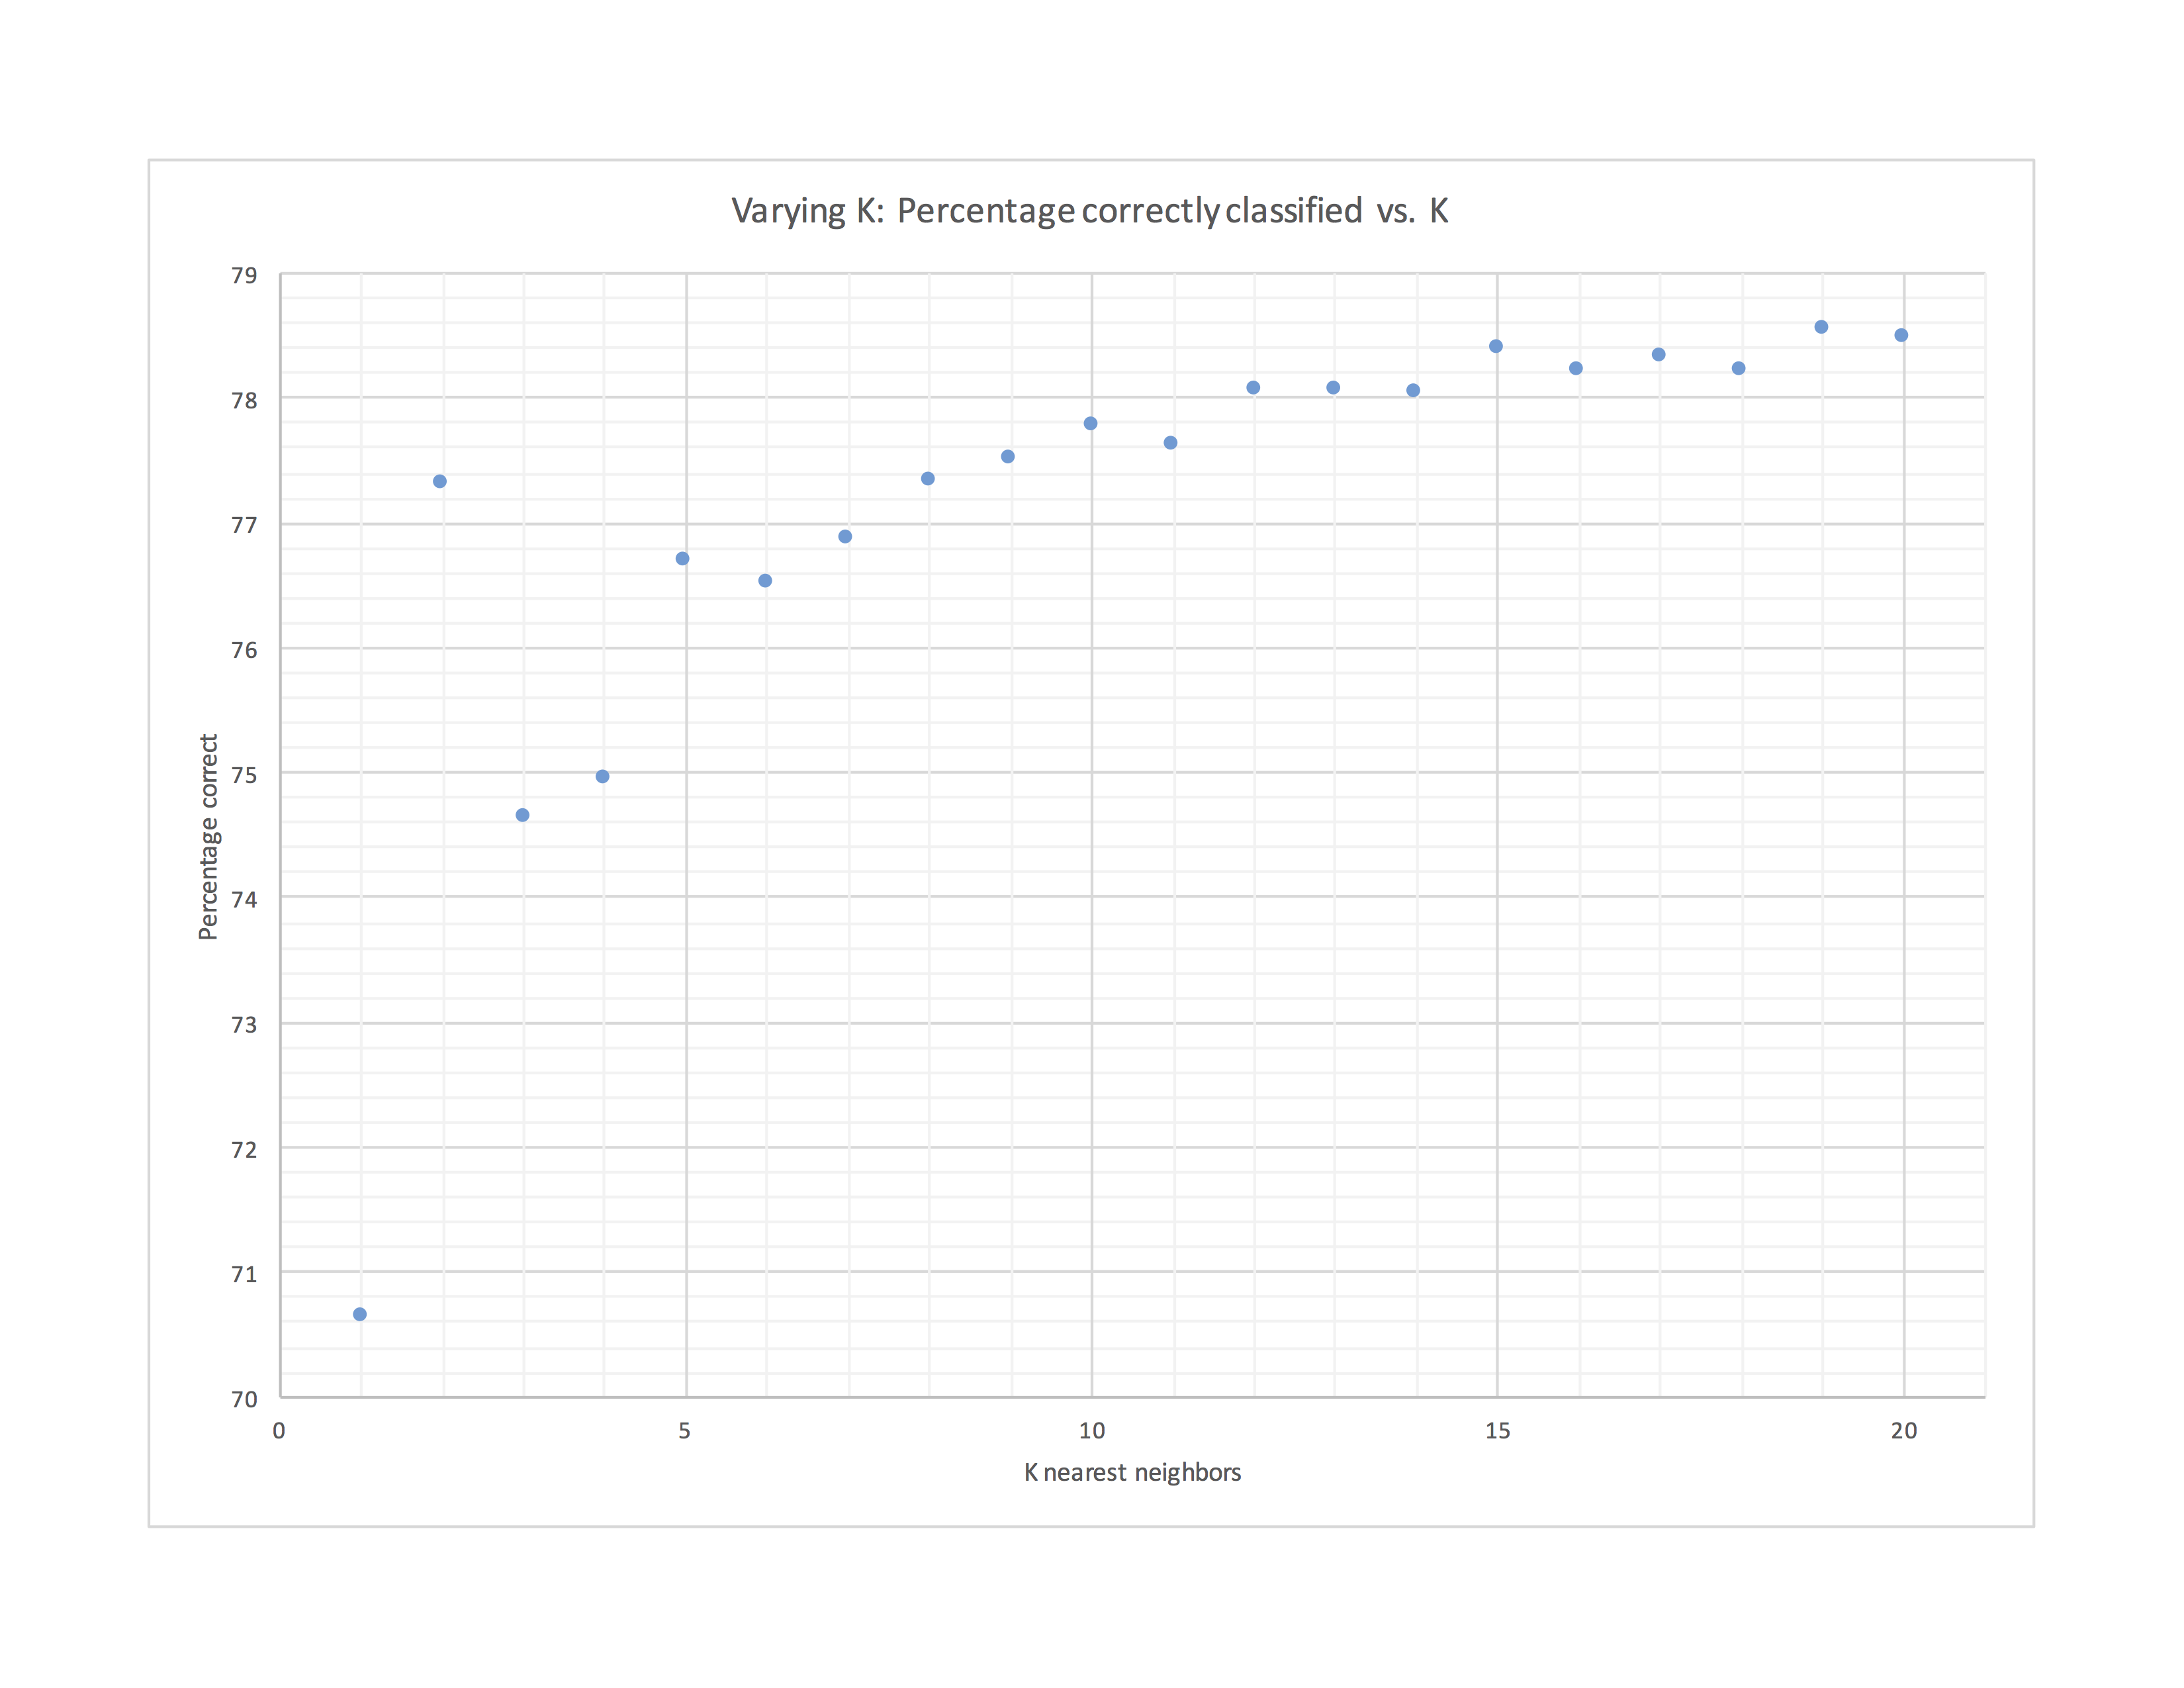
\includegraphics[width=1.0\textwidth]{varyingkKNN} % Include the image placeholder.png
\caption{Varying K and Tracking ClassifiedPercentage}
\end{center}
\end{figure}

This chart is interesting because it shows how we can, generally speaking, improve the performance of KNN by increasing the number of neighbors that are considered, especially for an application like this, where applying a euclidean distance between various pieces of information of two credit card holders does not intuitively make very much sense. We can see that as we increase the number of nearest neighbors considered from 1 to 20 the classification rate increases from about 70.5\% to 78.5\% (but it starts to plateau). However, we were more concerned about the timing implications of increasing K for the serial and parallel versions and will explore them below.
\clearpage
\begin{figure}[!htbp]
\begin{center}
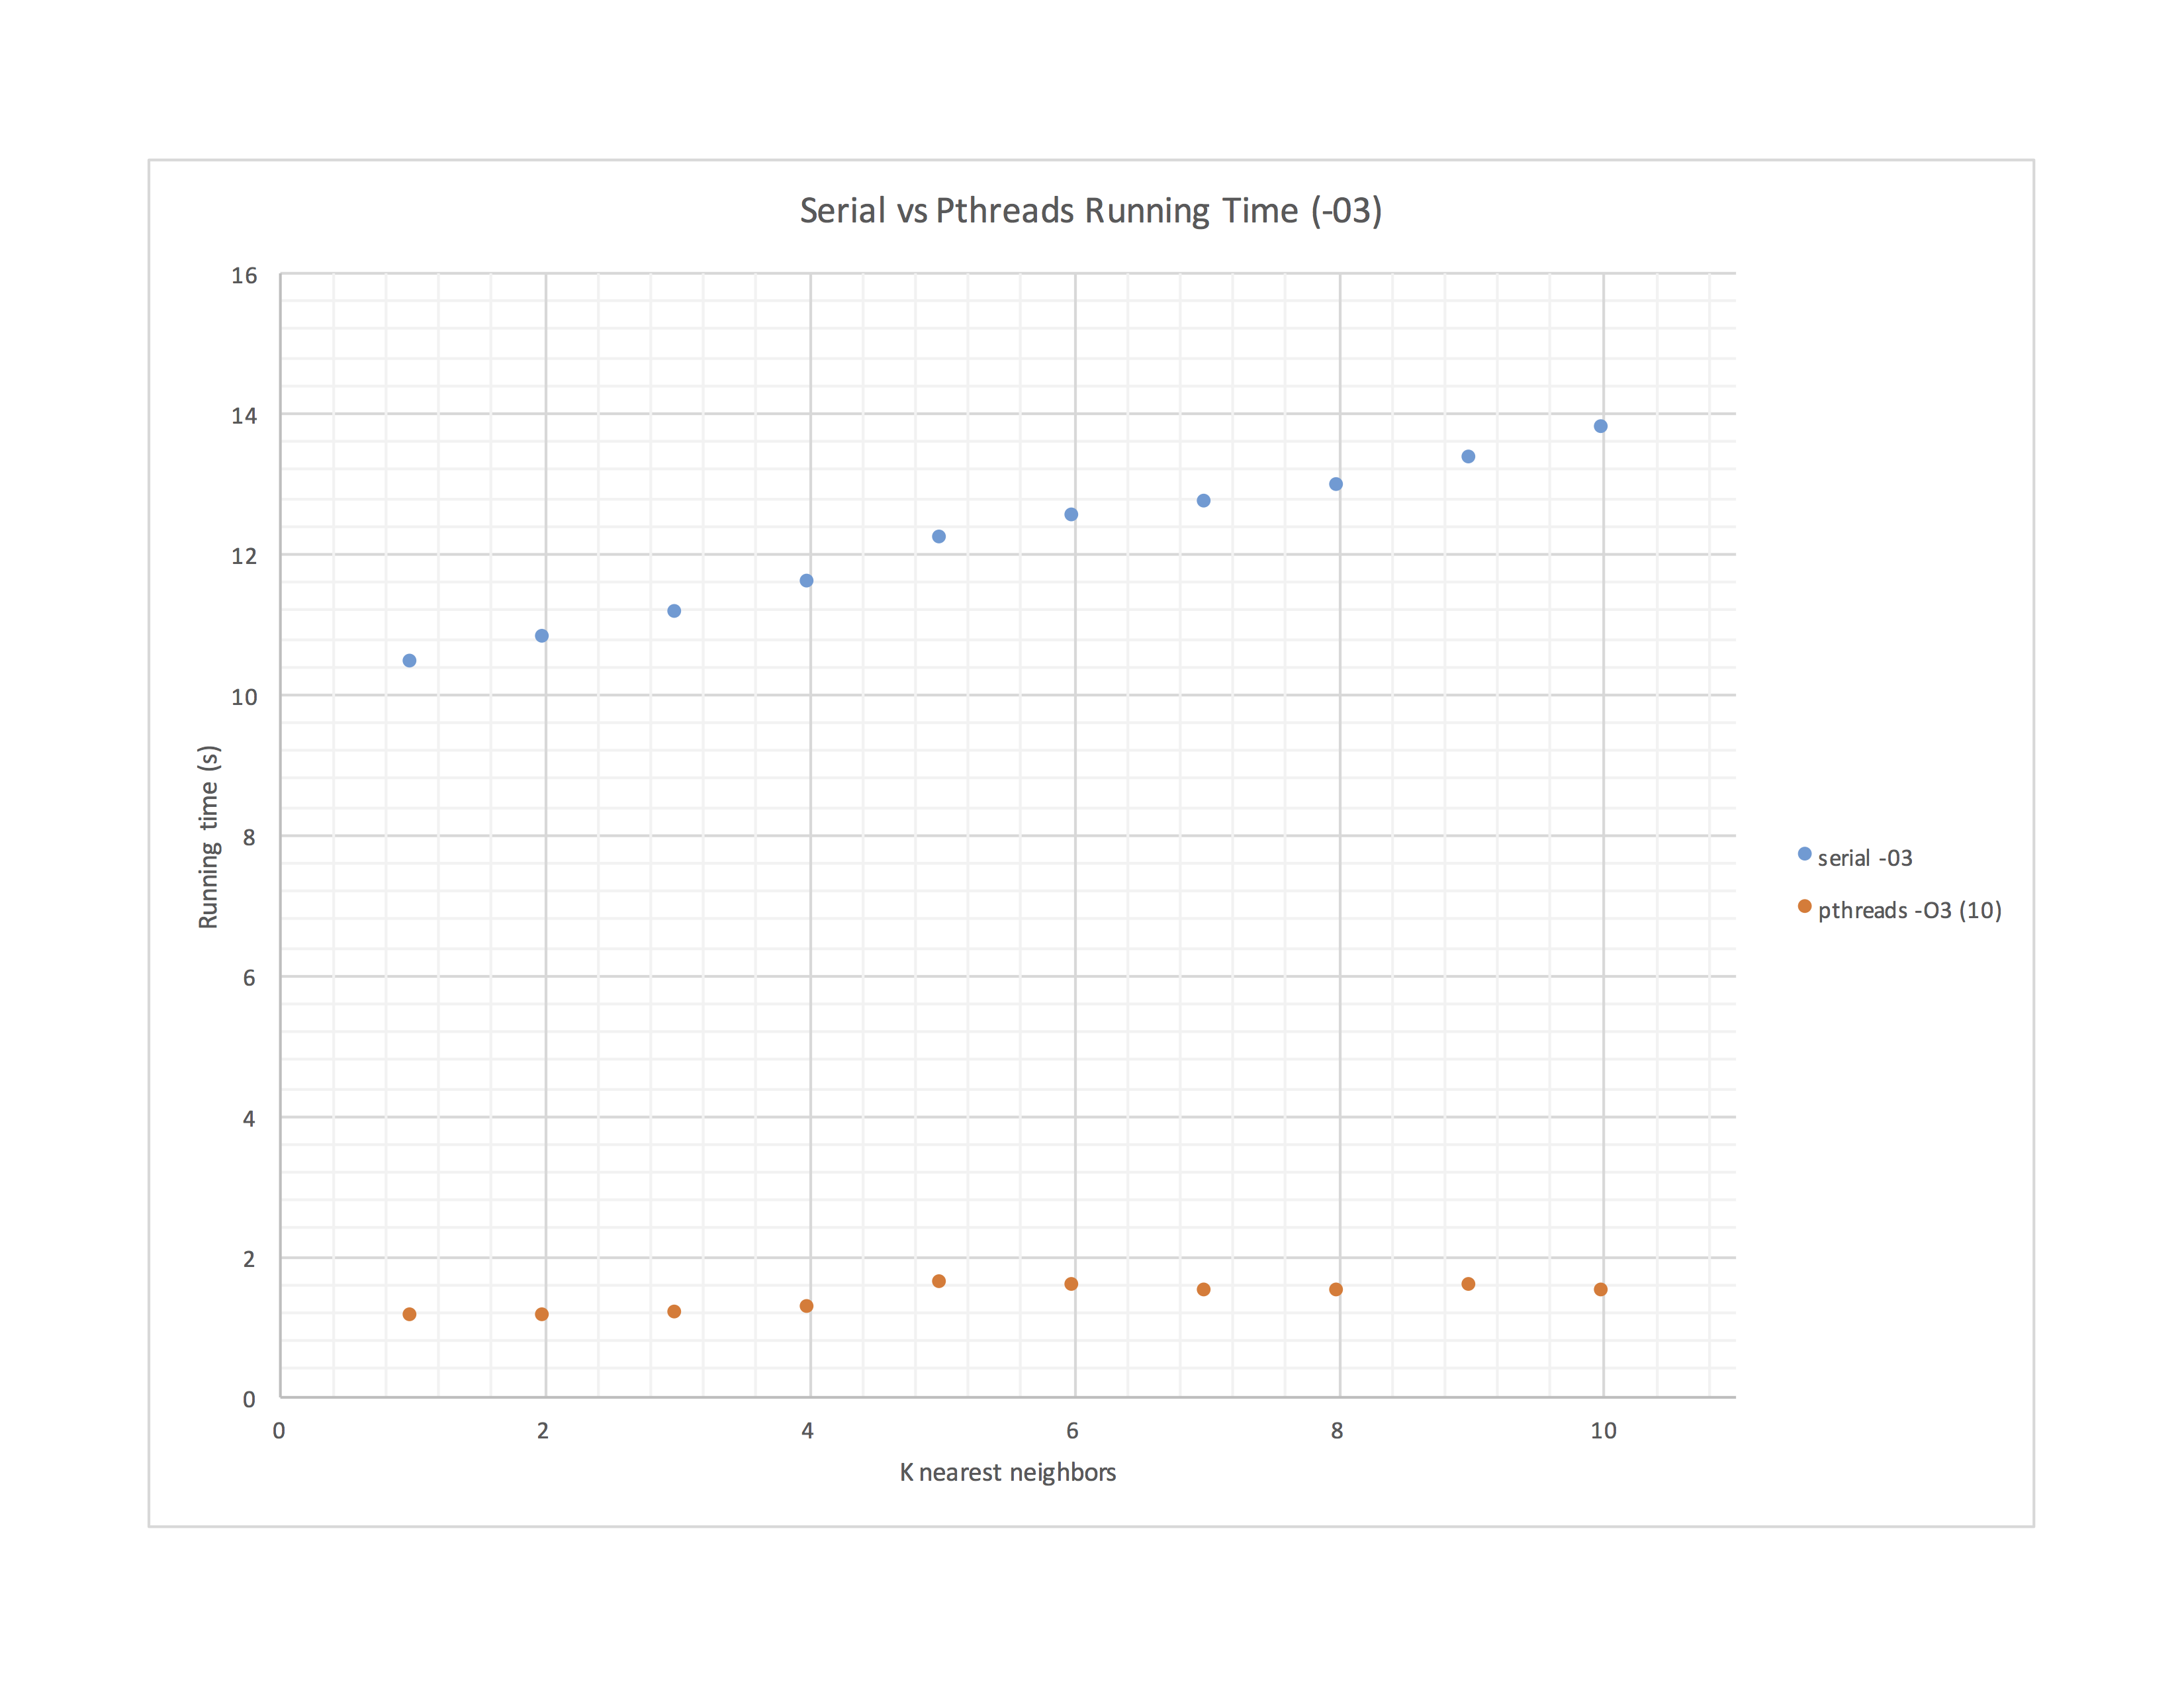
\includegraphics[width=1.0\textwidth]{runningtimeKNN} % Include the image placeholder.png
\caption{KNN: Serial vs PThreads Running Time (-O3)}
\end{center}
\end{figure}

In this chart we compare the running time of serial KNN versus our pthreads implementation running 10 threads with -O3 optimizations. We are looking at the total running time for both to classify 5000 data points using 25000 labeled points. Over these ten sizes for K, we saw an average speedup of 8.7 for the parallel implementation. \\

Perceptron actually performs far better on this dataset. We have implemented code that checks for convergence by saving a value which stores the minimum number missed accross all iterations. If this minimum is not surpassed after a set number of iterations, the perceptron algorithm stops.
\begin{verbatim}
 53         if (min_missed == -1 || sum_missed < min_missed) {
 54             min_missed = sum_missed;
 55             iters_since_best = 0;
 56             for (j = 0; j < x_dim; j++) {
 57                 w_converge[j] = w[j];
 58             }
 59         } else {
 60             if (iters_since_best >= 1000) {
 61                 for (j = 0; j < x_dim; j++) {
 62                     w[j] = w_converge[j];
 63                 }
 64                 break;
 65             }
 66             iters_since_best++;
 67         }
\end{verbatim}

Using this approach with 1000 iterations of no improvement as our threshold, we were able to classify 19434 of the 25000 training data points. Then, during testing we saw a classification rate of 78.8\% (3942 out of 5000). To find this weight vector took 1814 iterations total, so the best weight vector occurred at iteration 814 (followed by 1000 iterations of no improvement). Using our serial implementation of the perceptron algorithm, compiled with -O3 optimizations, we see a running of time of 2.1 seconds, significantly better than the running times of serial KNN and with a slightly better classification rate. This real world dataset shows that picking and tuning the right machine learning algorithm is going to be the most important thing to do to improve performance.
\clearpage
\section{Conclusion}
The goal of our work on this project was to take two very simple machine learning algorithms and optimize their performance through parallelization. The perceptron algorithm was particularly interesting because it is the building block of a neural net. The thinking goes that if you can improve the performance of a subcomponent drastically, then you can drastically improve the performance of the entire machine learning system. Parallelizing the perceptron algorithm is not straightforward, however, and requires considerable overhead to perform the necessary synchronizations between each iteration for both a multithreaded implementation and on the GPU. This is a case where parallelization at the neural net level, rather than attempting to parallelize this small component, is probably a better approach. \\
\\
We also wanted to compare and contrast the performance of a "lazy" algorithm like KNN, where testing and training occur at once with each classification, to an algorithm that separates the training and testing phase and generally finds some pattern within the data. An interesting dataset to look at was the credit card default dataset because KNN and perceptron could both be applied to it fairly straightforwardly (getting great results is another matter entirely, however). Ultimately, what we have learned from this comparison is that picking the right machine learning algorithm is far more important to acheive high correct classification rates than being able to process training data more quickly. For example, we could have had 60,000 data points in the UCI dataset instead of 30,000 but the perceptron algorithm would like still converge at the exact same point - the speed at which we processed the training data would not be significant to our overall success. However, if there is a proven method to solve some machine learning problem, whether it be face recognition or speech detection, and it is known to require huge amounts of training data (and that data is abundant), optimizing the training phase for maximum performance would provide significant and meaningful gains. \\

\end{document}